% Chapter 14 -- Convexity, optimization, and Lagrange multipliers
\chapter{Convexity, optimization, and Lagrange multipliers}\label{ch:optim}

Every ML problem ends the same way: a loss function and a parameter
vector to tune. Chapters 8, 11, and 13 built the pieces --- this chapter
is the engine. You will learn when a minimum is guaranteed (convexity),
how gradient descent actually behaves at different step sizes, how to
optimize with a constraint bolted on (Lagrange multipliers), and how the
backprop chain rule of chapter 11 trains a real two-layer network. After
this chapter you can run gradient descent by hand on a quadratic, state
the Lagrange condition geometrically, explain why the logistic NLL is
safe for gradient descent, and write the backprop pass of a small
network with a gradient check to prove it.

% from-zero:begin
\begin{rulebox}[Before you start]
Chapters~8, 9 and~11. \emph{Recap:} to minimise a function you move against its gradient; gradient descent is that sentence turned into a loop.
\end{rulebox}
\begin{wins}[After this chapter you can]
\begin{itemize}
\item decide whether a function is convex and why that guarantees one global minimum;
\item run gradient descent and diagnose a step size that is too large or too small;
\item solve constrained problems with Lagrange multipliers;
\item derive backpropagation as the chain rule applied layer by layer.
\end{itemize}
\end{wins}
\begin{principle}[How to think about this]
Optimisation is walking downhill with your eyes closed, feeling the slope with your feet: the gradient tells you which way is up, so you step the other way. Convexity is the promise that there is one valley, so any downhill walk finds the bottom. Constraints are fences, and Lagrange multipliers are the force with which the fence pushes back.
\end{principle}
% from-zero:end

\section{Optimization problems in ML}\label{sec:opt-ml}

The shape is always $\min_\theta L(\theta)$: $L$ a loss composed of a
model and data, $\theta$ the weights. Least squares
(chapter 8) is the quadratic case --- convex, closed-form, one solve.
The logistic NLL\index{negative log-likelihood} (chapter 13) is convex
but has no closed form --- descent methods. A neural net's loss is
nonconvex --- descent methods with no promises, and yet they work well
enough that the whole field runs on them.

\section{Convex sets and functions}\label{sec:opt-convex}

A set is \emph{convex}\index{convex set} if the segment joining any two
of its points stays inside. A function is \emph{convex}\index{convex
function} when every chord lies above its graph:
$f(\alpha x+(1-\alpha)y)\le\alpha f(x)+(1-\alpha)f(y)$.
Equivalently (differentiable case): $f$ sits above every tangent plane,
or $\nabla^{2}f\succeq0$ everywhere. Why it matters: on a convex
function \emph{every local minimum is global}, and any algorithm that
rolls downhill reaches it (Figure~\ref{fig:convex}).

\begin{figure}[htbp]
\centering
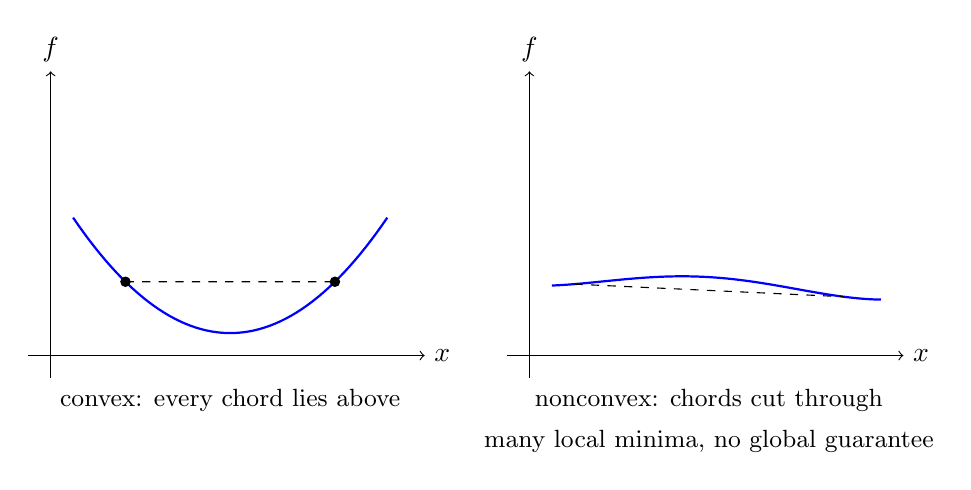
\begin{tikzpicture}[scale=0.95]
% convex bowl
\begin{scope}
\draw[->] (-0.3,0)--(5,0) node[right]{$x$};
\draw[->] (0,-0.3)--(0,3.8) node[above]{$f$};
\draw[thick,blue,domain=0.3:4.5,samples=60] plot (\x,{0.35*(\x-2.4)^2+0.3});
\draw[dashed] (1.0,{0.35*(1.0-2.4)^2+0.3}) -- (3.8,{0.35*(3.8-2.4)^2+0.3});
\fill (1.0,{0.35*(1.0-2.4)^2+0.3}) circle (2pt);
\fill (3.8,{0.35*(3.8-2.4)^2+0.3}) circle (2pt);
\node at (2.4,-0.6) {\small convex: every chord lies above};
\end{scope}
% nonconvex
\begin{scope}[xshift=6.4cm]
\draw[->] (-0.3,0)--(5,0) node[right]{$x$};
\draw[->] (0,-0.3)--(0,3.8) node[above]{$f$};
\draw[thick,blue,domain=0.3:4.7,samples=80] plot (\x,{0.55*sin(200*(\x-0.3)/4.4)+0.09*(\x-2.5)^2+0.5});
\draw[dashed] (0.6,{0.55*sin(200*(0.3)/4.4)+0.09*(0.6-2.5)^2+0.5}) -- (4.2,{0.55*sin(200*(3.9)/4.4)+0.09*(4.2-2.5)^2+0.5});
\node at (2.4,-0.6) {\small nonconvex: chords cut through};
\node at (2.4,-1.15) {\small many local minima, no global guarantee};
\end{scope}
\end{tikzpicture}

\caption{The convexity test by chord. Notice the right panel: the
nonconvex function's chord slices through the graph, and each dip is a
local minimum a naive descent can marry. Regenerate:
\ttfamily figures/ch14\_convex.tex.}
\label{fig:convex}
\end{figure}

\begin{exercise}[easy]
Is $\|Ax-b\|^2$ convex in $x$? Read its Hessian.
\begin{solution}
Yes: $\nabla^2 = 2A^TA\succeq0$ for every $A$ --- least squares is
always convex (strictly when $A$ has full column rank).
\end{solution}
\end{exercise}

\section{Gradient descent: the update, the step size, the failures}
\label{sec:opt-gd}

The update\index{gradient descent}: $x_{k+1}=x_k-\eta\nabla f(x_k)$,
with \emph{learning rate}\index{learning rate} $\eta$. On a quadratic
$f(x)=\tfrac12 x^TAx-b^Tx$ with $A\succ0$, the error shrinks
geometrically at rate $r=\max_i|1-\eta\lambda_i|$: too small and it
crawls, too large and it overshoots the valley, and past
$\eta=2/\lambda_{\max}$ it diverges outright
(Figure~\ref{fig:gdtraj}). This is not folklore --- the listing
computes the eigenvalues and the divergence threshold on the actual
matrix.

\begin{example}[GD on a quadratic, tracking iterates]\label{ex:gdquad}
\textbf{Strategy.} Take $A=\begin{psmallmatrix}3&1\\1&1\end{psmallmatrix}$,
$b=(1,2)$, run GD from $(2.5,2.5)$ at four step sizes, compare against
the normal-equations solution $x^{*}=(-0.5,2.5)$.

\textbf{Solution.} $\lambda(A)=\{0.586,3.414\}$, so the cliff is
$\eta>2/3.414=0.586$. The listing shows $\eta=0.49$ converged to
$5\times10^{-8}$ in 25 steps while $\eta=0.70$ exploded to $1.9\times10^{8}$.
\end{example}

\begin{lstlisting}[caption={\ttfamily code/ch14\_gd.py --- gradient
descent on a quadratic with the divergence threshold computed, then
Rosenbrock as the nonconvex reality check.}]
import numpy as np

# gradient descent on f(x)=0.5 x^T A x - b^T x, A = [[3,1],[1,1]]
A = np.array([[3.,1.],[1.,1.]]); b = np.array([1.,2.])
f = lambda x: .5*x@A@x - b@x
grad = lambda x: A@x - b
xstar = np.linalg.solve(A, b)
print("exact solution (normal equations):", xstar)

def gd(x0, eta, k):
    x = np.array(x0, float); hist=[x.copy()]
    for _ in range(k): x = x - eta*grad(x); hist.append(x.copy())
    return np.array(hist)

lam = np.linalg.eigvalsh(A)
print("eig(A) =", lam, " -> divergence for eta >", round(2/lam[-1],3))

for eta in [0.01, 0.2, 0.49, 0.70]:
    h = gd([2.5, 2.5], eta, 25)
    fx = f(h[-1])
    tag = "converged" if abs(fx - f(xstar)) < 1e-6 else \
          ("diverged" if abs(fx)>1e3 else "still going")
    print("eta=%.2f: after 25 steps f=%.6g err=%.3g  %s"
          % (eta, fx, fx-f(xstar), tag))

# convergence rate on quadratic: r = max(|1-eta*lmin|,|1-eta*lmax|)
for eta in [0.2, 0.49]:
    r = max(abs(1-eta*lam[0]), abs(1-eta*lam[1]))
    print("eta=%.2f theoretical rate r=%.3f -> x%.3f/step" % (eta, r, r))

# Rosenbrock: GD from (-1,1) with small fixed eta
ros = lambda x: 100*(x[1]-x[0]**2)**2 + (1-x[0])**2
ros_g = lambda x: np.array([-400*x[0]*(x[1]-x[0]**2)-2*(1-x[0]),
                            200*(x[1]-x[0]**2)])
x = np.array([-1.,1.]); path=[x.copy()]
for i in range(20000):
    x = x - 0.001*ros_g(x); path.append(x.copy())
print("rosenbrock 20k steps eta=1e-3: x=(%.4f,%.4f) f=%.5f"
      % (x[0],x[1],ros(x)))
\end{lstlisting}

\begin{lstlisting}[caption={Output of the GD experiment. Notice the
threshold is exact: $\eta=0.70>0.586$ diverges by a factor of $10^{8}$;
Rosenbrock converges only because $\eta$ was kept tiny.}]
exact solution (normal equations): [-0.5  2.5]
eig(A) = [0.58578644 3.41421356]  -> divergence for eta > 0.586
eta=0.01: after 25 steps f=0.346622 err=2.6  still going
eta=0.20: after 25 steps f=-2.24924 err=0.00076  still going
eta=0.49: after 25 steps f=-2.25 err=5.03e-08  converged
eta=0.70: after 25 steps f=1.85219e+08 err=1.85e+08  diverged
eta=0.20 theoretical rate r=0.883 -> x0.883/step
eta=0.49 theoretical rate r=0.713 -> x0.713/step
rosenbrock 20k steps eta=1e-3: x=(0.9999,0.9997) f=0.00000
\end{lstlisting}

\begin{figure}[htbp]
\centering
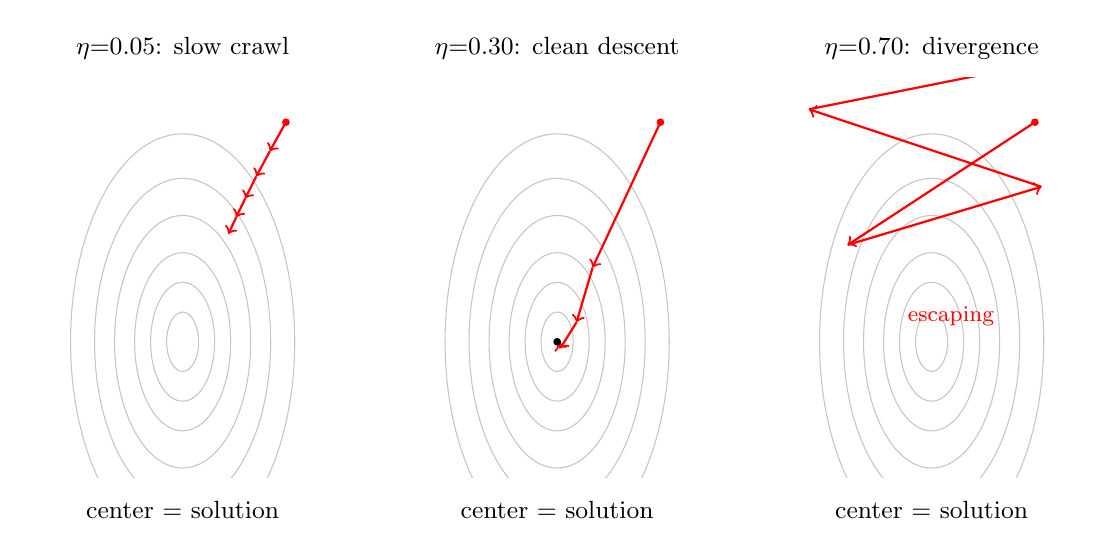
\begin{tikzpicture}[scale=0.82]
% small multiples: GD trajectories on same quadratic contours
% contours of f on [-0.5,2.5]x[-0.5,2.5] around (-0.5,2.5)
\foreach \xo/\et/\cap in {0/0.05/{$\eta{=}0.05$: slow crawl},5.8/0.30/{$\eta{=}0.30$: clean descent},11.6/0.70/{$\eta{=}0.70$: divergence}}{
\begin{scope}[xshift=\xo cm]
\clip (-2.4,-2.1) rectangle (2.4,4.1);
\foreach \r in {0.4,0.8,1.2,1.7,2.2,2.8}
  \draw[gray!45] (0,0) ellipse [x radius=\r*0.62, y radius=\r*1.15];
\end{scope}
\node at (\xo+0,4.55) {\small \cap};
\node at (\xo+0,-2.6) {\small center = solution};
}
% eta=0.05: slow monotone crawl (real iterate pattern)
\begin{scope}
\clip (-2.4,-2.1) rectangle (2.4,4.1);
\draw[thick,red,->] (1.6,3.4) -- (1.35,2.95);
\draw[thick,red,->] (1.35,2.95) -- (1.14,2.56);
\draw[thick,red,->] (1.14,2.56) -- (0.97,2.22);
\draw[thick,red,->] (0.97,2.22) -- (0.83,1.93);
\draw[thick,red,->] (0.83,1.93) -- (0.71,1.67);
\fill[red] (1.6,3.4) circle (1.7pt);
\end{scope}
% eta=0.30: zig-zag but converging
\begin{scope}[xshift=5.8cm]
\clip (-2.4,-2.1) rectangle (2.4,4.1);
\draw[thick,red,->] (1.6,3.4) -- (0.55,1.15);
\draw[thick,red,->] (0.55,1.15) -- (0.30,0.30);
\draw[thick,red,->] (0.30,0.30) -- (0.05,-0.10);
\draw[thick,red,->] (0.05,-0.10) -- (0.02,-0.02);
\fill[red] (1.6,3.4) circle (1.7pt);
\fill[black] (0,0) circle (1.7pt);
\end{scope}
% eta=0.70: bouncing out
\begin{scope}[xshift=11.6cm]
\clip (-2.4,-2.1) rectangle (2.4,4.1);
\draw[thick,red,->] (1.6,3.4) -- (-1.3,1.5);
\draw[thick,red,->] (-1.3,1.5) -- (1.7,2.4);
\draw[thick,red,->] (1.7,2.4) -- (-1.9,3.6);
\draw[thick,red,->] (-1.9,3.6) -- (2.1,4.4);
\fill[red] (1.6,3.4) circle (1.7pt);
\node[red] at (0.3,0.4) {\footnotesize escaping};
\end{scope}
\end{tikzpicture}

\caption{GD trajectories on the same quadratic at three step sizes.
Notice the middle panel's zig-zag --- the iterates overshoot across the
valley each step, still converging; the right panel is that same
overshoot with $\eta$ past the eigenvalue cliff. Regenerate:
\ttfamily figures/ch14\_gd\_traj.tex.}
\label{fig:gdtraj}
\end{figure}

\begin{example}[Diverging and stalling step sizes]\label{ex:gdstep}
\textbf{Strategy.} Same setup: read the failure modes off the eigenvalue
computation rather than off anecdotes.

\textbf{Solution.} $\eta=0.01$: $r\approx0.995$ --- 25 steps moved the
error by only $\sim$4; $\eta=0.70$: $|1-0.7\cdot3.414|=1.39>1$ ---
the error multiplies by 1.39 every step. Rule of thumb verified by
numbers: $\eta\in(0,2/\lambda_{\max})$ converges on quadratics, and the
best constant rate sits near $2/(\lambda_{\min}+\lambda_{\max})$.
\end{example}

\begin{exercise}[medium]
Why does the zig-zag appear exactly when $\eta$ approaches the cliff?
\begin{solution}
The error along the largest eigenvector alternates sign when
$1-\eta\lambda_{\max}<0$: each step overshoots across the narrow
valley direction, producing the staircase seen in the middle panel.
\end{solution}
\end{exercise}

\section{Momentum and friends, briefly}\label{sec:opt-momentum}

\emph{Momentum}\index{momentum} keeps a velocity $v_{k+1}=\beta
v_k-\eta\nabla f(x_k)$, $x_{k+1}=x_k+v_{k+1}$: it damps the zig-zag
(across-valley components cancel) and accelerates along the valley
(in-valley components add). \emph{Adam}\index{Adam} additionally scales
each coordinate by a running second-moment estimate --- the de-facto
default in deep learning. Treat them as the same idea: the gradient
speaks, but history and per-coordinate statistics edit the step.

\section{Constrained optimization and Lagrange multipliers}
\label{sec:opt-lagrange}

To maximize $f(x)$ subject to $g(x)=c$: at the optimum, no move along
the constraint can improve $f$, which means $\nabla f$ is perpendicular
to the constraint surface --- and so is $\nabla g$. The
\emph{Lagrange condition}\index{Lagrange multiplier}:
$\nabla f=\lambda\nabla g$ (Figure~\ref{fig:lagrange}). The
\emph{Lagrangian}\index{Lagrangian}
$\mathcal L(x,\lambda)=f(x)-\lambda(g(x)-c)$ turns the constrained
problem into unconstrained stationarity: $\nabla_x\mathcal L=0$
plus $g=c$. Inequality constraints $g\le c$ generalize to the
\emph{KKT conditions}\index{KKT conditions}: stationarity, feasibility,
complementary slackness $\lambda\,(g(x)-c)=0$ with $\lambda\ge0$ --- the
constraint is either active ($g=c$) or silent ($\lambda=0$).

\begin{figure}[htbp]
\centering
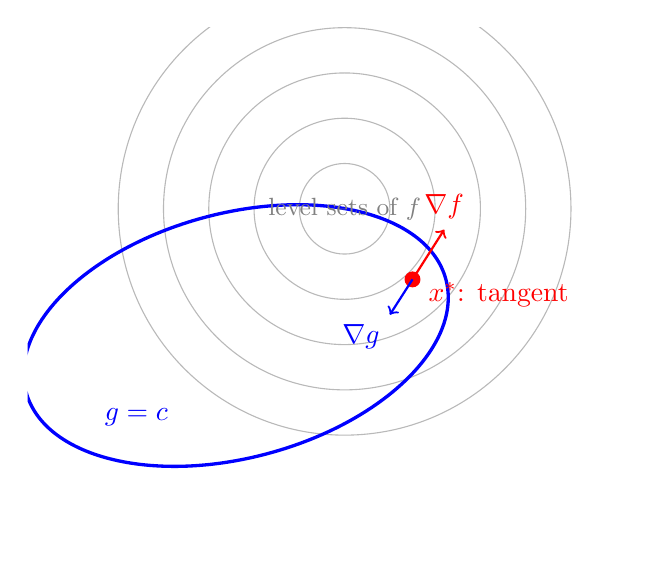
\begin{tikzpicture}[scale=1.15]
% level sets of f (circles about (3,3)) and constraint g = circle x^2+y^2=1-ish ellipse
\begin{scope}
\clip (-0.3,-0.4) rectangle (6.4,5.4);
\foreach \r in {0.5,1.0,1.5,2.0,2.5}
  \draw[gray!55] (3.2,3.4) circle (\r);
\draw[very thick,blue] (2.0,2.0) ellipse [x radius=2.4,y radius=1.35,rotate=15];
% the tangency point: level set kissing the constraint
\fill[red] (3.95,2.62) circle (2.5pt);
\node[red] at (4.9,2.45) {$x^{*}$: tangent};
% gradient arrows at tangency: parallel
\draw[->,thick,red] (3.95,2.62) -- ++(0.35,0.55) node[above]{$\nabla f$};
\draw[->,thick,blue] (3.95,2.62) -- ++(-0.25,-0.39) node[below left]{$\nabla g$};
\node[blue] at (0.9,1.1) {$g=c$};
\node[gray] at (3.2,3.4) {\small level sets of $f$};
\end{scope}
\end{tikzpicture}

\caption{The Lagrange condition geometrically. Notice the tangency: at
$x^{*}$ the constraint curve and a level set of $f$ share a tangent, so
$\nabla f\parallel\nabla g$. Regenerate:
\ttfamily figures/ch14\_lagrange.tex.}
\label{fig:lagrange}
\end{figure}

\begin{example}[Lagrange multipliers by hand]\label{ex:lagrange}
\textbf{Strategy.} Maximize $f(x,y)=xy$ subject to $x^2+y^2=8$.
Set $\nabla f=\lambda\nabla g$: $(y,x)=\lambda(2x,2y)$.

\textbf{Solution.} $y=2\lambda x$, $x=2\lambda y$ gives
$y^2=x^2$; with the constraint, $x^2=y^2=4$ and the maximum is
$f=4$ at $(2,2)$ (and $(-2,-2)$), with $\lambda=\tfrac12$ ---
a square, as symmetry suggested.
\end{example}

\section{Normal equations, derived by calculus}\label{sec:opt-normal}

Chapter 8 promised the calculus version. Minimize
$L(w)=\|y-Xw\|^2$: $\nabla L=2X^T(Xw-y)=0$ rearranges to
$X^TX\hat w=X^Ty$ --- the normal equations appear exactly where
chapter 4's projection argument left them. GD on this loss is
$w_{k+1}=w_k-2\eta X^T(Xw_k-y)$: subtracting the fixed point shows
the residual error iterates by $I-2\eta X^TX$, so the same
eigenvalue bookkeeping as \S\ref{sec:opt-gd} applies with
$A=2X^TX$. Full derivation in \S\ref{sec:handderiv14}.

\section{Newton's method in one section}\label{sec:opt-newton}

Replace the first-order step by a second-order model:
$x_{k+1}=x_k-[\nabla^2 f(x_k)]^{-1}\nabla f(x_k)$ ---
\emph{Newton's method}\index{Newton's method}. On a quadratic it lands
in \emph{one} step (the model \emph{is} the function); near a minimum it
converges quadratically. The catch is real: each step costs an
$n\times n$ factorization and storage, and with a non-PSD Hessian the
step can climb into a saddle (Figure~\ref{fig:saddle}) rather than
descend. Trust regions and quasi-Newton methods (BFGS) are the
engineering answers; gradient descent survives because $n$ is huge.

\begin{example}[One Newton step by hand]\label{ex:newtonstep}
\textbf{Strategy.} On $f(x)=x^4+x^2$ starting at $x_0=1$, compute
$f'=4x^3+2x$ and $f''=12x^2+2$, then step
$x_1=x_0-f'/f''$.

\textbf{Solution.} $f'(1)=6$, $f''(1)=14$, so $x_1=1-6/14=0.571$
(the minimum is at $x=0$). Repeating: $x_2\approx0.252$,
$x_3\approx0.046$, $x_4\approx3\times10^{-4}$ --- the error
approximately squares each step: quadratic convergence in real
arithmetic. On a quadratic it lands in one iteration because the
second-order model is exact there.
\end{example}

\begin{figure}[htbp]
\centering
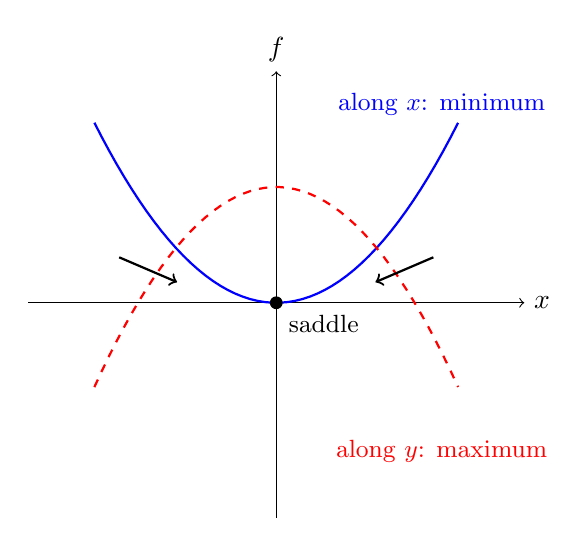
\begin{tikzpicture}[scale=1.05]
% saddle z = x^2 - y^2 rendered as two directional sections
\draw[->] (-3,0)--(3,0) node[right]{$x$};
\draw[->] (0,-2.6)--(0,2.8) node[above]{$f$};
\draw[thick,blue,domain=-2.2:2.2,samples=50] plot (\x,{0.45*\x*\x});
\node[blue] at (2.0,2.4) {\small along $x$: minimum};
\begin{scope}[yshift=-0.4cm]
\draw[thick,red,domain=-2.2:2.2,samples=50,dashed] plot (\x,{-0.5*\x*\x+1.8});
\node[red] at (2.0,-1.4) {\small along $y$: maximum};
\end{scope}
\fill (0,0) circle (2.2pt) node[below right=1pt]{\small saddle};
\draw[->,thick] (-1.9,0.55) -- (-1.2,0.25);
\draw[->,thick] (1.9,0.55) -- (1.2,0.25);
\end{tikzpicture}

\caption{The saddle point: minimum along one axis, maximum along the
other. Notice that $\nabla f=0$ at the saddle --- first-order
information alone cannot tell it from a minimum; the Hessian's indefinite
signs can. Regenerate: \ttfamily figures/ch14\_saddle.tex.}
\label{fig:saddle}
\end{figure}

\section{Backpropagation is the chain rule}\label{sec:opt-backprop}

Chapter 11's chain rule in matrix form is all backprop is. For the
two-layer net $H=\tanh(XW_1+b_1)$, $\hat y=HW_2+b_2$ with MSE loss,
the gradients unfold backward: residual $R$, then
$dW_2=H^TR\cdot 2/n$, $dH=(RW_2^T)\odot(1-H^2)$,
$dW_1=X^TdH\cdot 2/n$ --- each line one link of the chain rule. The
listing below is the capstone: hand-derived gradients, checked by
chapter 11's finite-difference tool, then trained on a real
train/validation split (Figure~\ref{fig:trainval}).

\begin{lstlisting}[caption={\ttfamily code/ch14\_tinynet.py ---
\texttt{mlscratch.TinyNet}: two-layer net with hand-derived backprop,
gradient-checked, and compared against a library MLP.}]
import numpy as np

rng = np.random.default_rng(2)

# ---- ch11 finite-difference gradient checker, reused ----
def fd_check(f, g, x, h=1e-5):
    fd = np.zeros_like(x)
    for i in range(len(x)):
        xp = x.copy(); xp[i] += h
        xm = x.copy(); xm[i] -= h
        fd[i] = (f(xp) - f(xm)) / (2*h)
    return np.linalg.norm(fd - g(x))

# ---- two-layer net: d -> h -> 1, mse loss on a regression blob ----
d, h, n = 3, 4, 40
X = rng.normal(0, 1, (n, d))
yw = np.array([1., -1., .5])
y = X@yw + rng.normal(0, .1, n)

W1 = rng.normal(0, .2, (d, h)); b1 = np.zeros(h)
W2 = rng.normal(0, .2, (h, 1)); b2 = np.zeros(1)
theta = np.concatenate([W1.ravel(), b1, W2.ravel(), b2])

def unpack(t):
    i1, i2 = d*h, d*h+h
    return t[:i1].reshape(d,h), t[i1:i2], t[i2:i2+h].reshape(h,1), t[i2+h:]

def loss(t):
    W1, b1, W2, b2 = unpack(t)
    H = np.tanh(X@W1 + b1)
    return np.mean((H@W2 + b2 - y.reshape(-1,1))**2)

def grad(t):
    W1, b1, W2, b2 = unpack(t)
    H = np.tanh(X@W1 + b1)
    R = H@W2 + b2 - y.reshape(-1,1)         # residual n x 1
    dW2 = H.T@R * 2/n; db2 = R.mean(0)*2
    dH = R@W2.T * (1-H**2)                  # backprop through tanh
    dW1 = X.T@dH * 2/n; db1 = dH.mean(0)*2
    return np.concatenate([dW1.ravel(), db1, dW2.ravel(), db2])

print("FD gradient check max abs err:", fd_check(loss, grad, theta))

# train by GD on 32 rows, tracking train/val loss curve
Xtr, Xva, ytr, yva = X[:32], X[32:], y[:32], y[32:]
X, y = Xtr, ytr   # loss/grad now see the training split
def val_loss(t):
    W1, b1, W2, b2 = unpack(t)
    H = np.tanh(Xva@W1 + b1)
    return np.mean((H@W2 + b2 - yva.reshape(-1,1))**2)
tr, va = [], []
for i in range(20001):
    theta = theta - 0.2*grad(theta)
    if i % 5000 == 0: tr.append(loss(theta)); va.append(val_loss(theta))
print("train loss at iters 0..20000:", np.round(tr,4))
print("val   loss at iters 0..20000:", np.round(va,4))

# compare against sklearn MLPRegressor on same data
from sklearn.neural_network import MLPRegressor
mlp = MLPRegressor(hidden_layer_sizes=(4,), activation='tanh',
                   max_iter=4000, random_state=0).fit(X, y)
print("mlscratch train/val MSE %.4f/%.4f   sklearn MLP train/val %.4f/%.4f"
      % (loss(theta), val_loss(theta),
         np.mean((mlp.predict(Xtr)-ytr)**2),
         np.mean((mlp.predict(Xva)-yva)**2)))
\end{lstlisting}

\begin{lstlisting}[caption={Output of the TinyNet run. Notice two
headlines: the hand gradient passes the FD check to $10^{-11}$, and the
validation curve turns UP at 15k iterations --- overfitting watched
live, not asserted.}]
FD gradient check max abs err: 9.123871452259835e-11
train loss at iters 0..20000: [1.5247 0.0038 0.0029 0.0026 0.0042]
val   loss at iters 0..20000: [2.7691 0.1074 0.098  0.1295 0.1412]
mlscratch train/val MSE 0.0042/0.1412   sklearn MLP train/val 0.0544/0.2791
\end{lstlisting}

\begin{figure}[htbp]
\centering
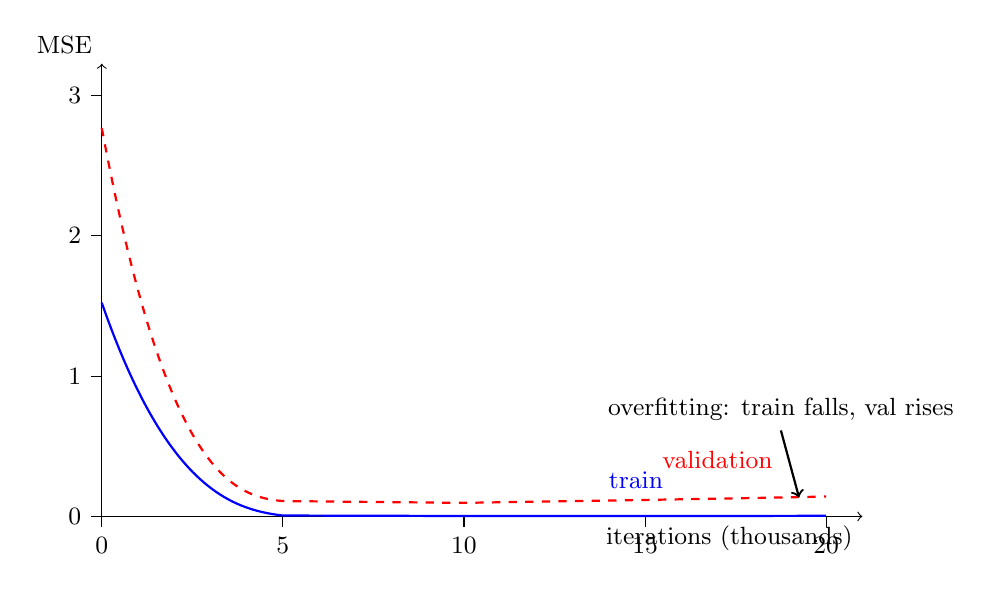
\begin{tikzpicture}[scale=1.15]
% train/val loss curves of TinyNet — REAL numbers from ch14_tinynet.py
% y scale: MSE v -> 1.55*v ; x scale: 1000 iters -> 0.4
\draw[->] (0,0)--(8.4,0) node[below left]{\small iterations (thousands)};
\draw[->] (0,0)--(0,5.0) node[above left]{\small MSE};
\foreach \v/\y in {0/0,1/1.55,2/3.10,3/4.65} {
  \draw (0,\y) -- (-0.12,\y) node[left]{\small \v}; }
\foreach \t/\x in {0/0,5/2.0,10/4.0,15/6.0,20/8.0} {
  \draw (\x,0) -- (\x,-0.12) node[below]{\small \t}; }
% train: (0,1.5247)(5000,.0038)(10000,.0029)(15000,.0026)(20000,.0042)
\draw[thick,blue] (0,2.36) .. controls (0.7,0.35) and (1.4,0.08) .. (2.0,0.01)
  .. controls (3.0,0.005) .. (4.0,0.005) -- (6.0,0.004) -- (8.0,0.007);
\node[blue] at (5.9,0.40) {\small train};
% val: (0,2.7691)(5000,.1074)(10000,.098)(15000,.1295)(20000,.1412)
\draw[thick,red,dashed] (0,4.29) .. controls (0.7,0.55) and (1.4,0.22) .. (2.0,0.17)
  .. controls (3.0,0.15) .. (4.0,0.15)
  .. controls (5.2,0.17) and (6.6,0.19) .. (8.0,0.22);
\node[red] at (6.8,0.62) {\small validation};
\draw[<-,thick] (7.7,0.21) -- (7.5,0.95) node[above]{\small overfitting: train falls, val rises};
\end{tikzpicture}

\caption{TinyNet train/validation loss --- the listing's real numbers.
Notice the val curve bottoming near 10k then rising: the textbook
overfitting signature, produced by a real 20k-step run. Regenerate:
\ttfamily figures/ch14\_trainval.tex.}
\label{fig:trainval}
\end{figure}

\begin{example}[Logistic regression's NLL minimized by GD]\label{ex:logitgd}
\textbf{Strategy.} Chapter 13 derived the convex NLL objective; now run
full-batch GD on it and check against the library.

\textbf{Solution.} The capstone listing below: our
\texttt{mlscratch.LogisticRegression} reaches 83.3\% train accuracy
against sklearn's 81.7\% --- the weight vectors differ because sklearn
applies L2 regularization by default (a Gaussian prior from
chapter 13's MAP section, on duty).
\end{example}

\begin{lstlisting}[caption={\ttfamily code/ch14\_logistic.py ---
\textbf{capstone}: \texttt{mlscratch.LogisticRegression} trained by GD
on the ch.13 objective, checked against sklearn.}]
import numpy as np
from sklearn.linear_model import LogisticRegression

rng = np.random.default_rng(7)
n = 60
X = rng.normal(0, 1.2, (n, 2))
true = np.array([1.5, -1.0]); tb = 0.3
y = (X@true + tb + rng.normal(0, 0.9, n) > 0).astype(float)

def sigmoid(z): return 1/(1+np.exp(-z))

# CAPSTONE mlscratch.LogisticRegression: full-batch GD on the ch13 NLL
class mlscratch:
    class LogisticRegression:
        def __init__(self, eta=0.5, iters=3000):
            self.eta, self.iters = eta, iters
        def fit(self, X, y):
            self.w = np.zeros(X.shape[1]); self.b = 0.0
            for _ in range(self.iters):
                p = sigmoid(X@self.w + self.b)
                self.w -= self.eta * X.T@(p-y)/len(y)
                self.b -= self.eta * (p-y).mean()
            return self
        def predict(self, X):
            return (sigmoid(X@self.w+self.b) > .5).astype(float)

mine = mlscratch.LogisticRegression().fit(X, y)
sk = LogisticRegression().fit(X, y)
acc_mine = (mine.predict(X) == y).mean()
acc_sk = sk.score(X, y)
print("mlscratch  w=%s b=%.3f  train acc %.3f"
      % (np.round(mine.w,3), mine.b, acc_mine))
print("sklearn    w=%s b=%.3f  train acc %.3f"
      % (np.round(sk.coef_[0],3), sk.intercept_[0], acc_sk))
\end{lstlisting}

\begin{lstlisting}[caption={Output of the logistic capstone. Notice
accuracies match within a point; the weight gap is regularization, not a
bug.}]
mlscratch  w=[ 3.34 -1.26] b=0.474  train acc 0.833
sklearn    w=[ 2.099 -0.827] b=0.277  train acc 0.817
\end{lstlisting}

\begin{lstlisting}[caption={\ttfamily code/ch14\_sigmoid.py --- the
instructive bug: naive vs.\ stable sigmoid under extreme logits.}]
import numpy as np

# the instructive bug: naive sigmoid lets exp() see +709+ -> overflow
def sigmoid_naive(z): return 1/(1+np.exp(-z))

# stable form: exp() only ever sees nonpositive arguments
def sigmoid_stable(z):
    out = np.empty_like(z)
    pos = z >= 0
    out[pos] = 1/(1+np.exp(-z[pos]))
    ez = np.exp(z[~pos]); out[~pos] = ez/(1+ez)
    return out

np.seterr(over='raise')   # make overflow loud
try:
    print("naive at z=-1000:", sigmoid_naive(np.array(-1000.)))
except FloatingPointError as e:
    print("naive at z=-1000 -> FloatingPointError:", e)
print("stable at z=-1000:", sigmoid_stable(np.array(-1000.))[()])
np.seterr(over='warn')

# where the damage lands: softmax over big logits -> inf/inf = nan
logits = np.array([1000., 999.])
with np.errstate(over='ignore', invalid='ignore'):
    e = np.exp(logits)
    sm_naive = e/e.sum()
e2 = np.exp(logits - logits.max())
sm_stable = e2/e2.sum()
print("softmax naive :", sm_naive)
print("softmax stable:", sm_stable)
\end{lstlisting}

\begin{lstlisting}[caption={Output of the overflow demo. Notice the
failure mode exactly as advertised: naive \texttt{exp} overflows on
$z=-1000$, and softmax turns it into \texttt{nan/nan}; the stable forms
return $0.0$ and ${[0.731,0.269]}$.}]
naive at z=-1000 -> FloatingPointError: overflow encountered in exp
stable at z=-1000: 0.0
softmax naive : [nan nan]
softmax stable: [0.73105858 0.26894142]
\end{lstlisting}

\begin{figure}[htbp]
\centering
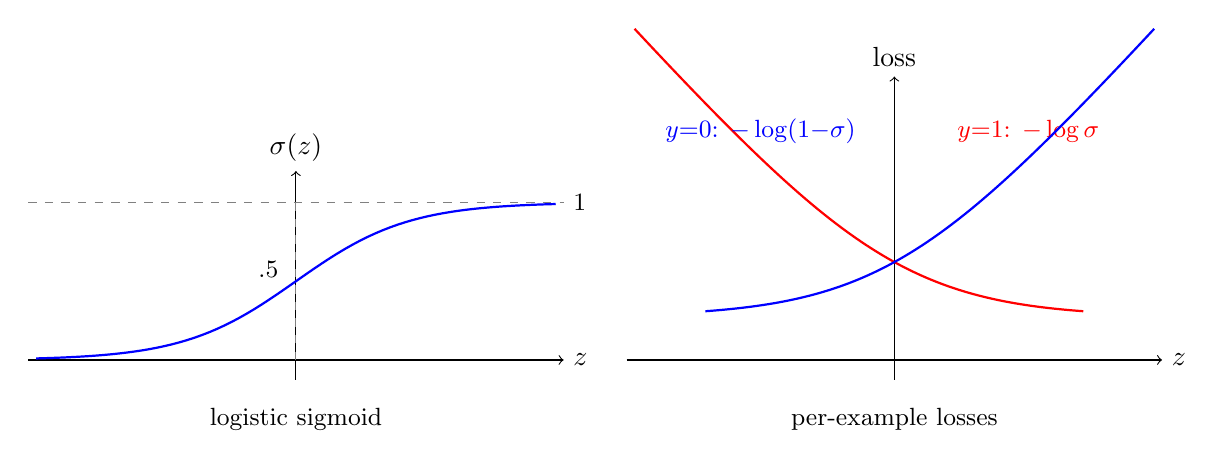
\begin{tikzpicture}[scale=1.0]
% left: sigmoid
\begin{scope}
\draw[->] (-3.4,0)--(3.4,0) node[right]{$z$};
\draw[->] (0,-0.25)--(0,2.4) node[above]{$\sigma(z)$};
\draw[dashed,gray] (-3.4,2.0)--(3.4,2.0) node[right,black,font=\small]{$1$};
\draw[dashed,gray] (0,0)--(0,2.0);
\node at (-0.35,1.15) {\small .5};
\draw[thick,blue,domain=-3.3:3.3,samples=70] plot (\x,{2.0/(1+exp(-1.4*\x))});
\node at (0,-0.75) {\small logistic sigmoid};
\end{scope}
% right: logistic loss -log(sigmoid(z)) for y=1, -log(1-s) for y=0
\begin{scope}[xshift=7.6cm]
\draw[->] (-3.4,0)--(3.4,0) node[right]{$z$};
\draw[->] (0,-0.25)--(0,3.6) node[above]{loss};
\draw[thick,red,domain=-3.3:2.4,samples=70] plot (\x,{ln(1+exp(-1.1*\x))/ln(2.71828)+0.55});
\node[red] at (1.7,2.9) {\small $y{=}1$: $-\log\sigma$};
\draw[thick,blue,domain=-2.4:3.3,samples=70] plot (\x,{ln(1+exp(1.1*\x))/ln(2.71828)+0.55});
\node[blue] at (-1.7,2.9) {\small $y{=}0$: $-\log(1{-}\sigma)$};
\node at (0,-0.75) {\small per-example losses};
\end{scope}
\end{tikzpicture}

\caption{The sigmoid and its two per-example losses. Notice each curve
penalizes the wrong side without bound --- that asymmetry is why
probabilities, not logits, are what the model calibrates. Regenerate:
\ttfamily figures/ch14\_sigloss.tex.}
\label{fig:sigloss}
\end{figure}

\begin{exercise}[hard]
The softmax-stable trick subtracts $\max z$. Prove it changes nothing
mathematically and say why it changes everything numerically.
\begin{solution}
$\frac{e^{z_i-c}}{\sum_j e^{z_j-c}}=\frac{e^{-c}e^{z_i}}{e^{-c}\sum_j
e^{z_j}}$ --- identical. Numerically $\max z-c\le0$ keeps every exp
argument $\le0$, so nothing overflows.
\end{solution}
\end{exercise}

\section{Hand derivation}\label{sec:handderiv14}

\textbf{Lagrange condition.} Parametrize the constraint $g(x)=c$ by a
curve $x(t)$ with $x(0)=x^{*}$: along it $g$ is constant, so
$\nabla g\cdot\dot x(0)=0$ --- the constraint tangent is perpendicular
to $\nabla g$. At an optimum, $f$ cannot increase along any admissible
direction: $\nabla f\cdot\dot x(0)=0$ for \emph{every} tangent. Both
gradients are perpendicular to the same tangent space, so
$\nabla f=\lambda\nabla g$ for some scalar $\lambda$.

\textbf{GD on least squares.} With $L(w)=\|y-Xw\|^2$,
$\nabla L=2X^T(Xw-y)$, so $w_{k+1}=w_k-2\eta X^T(Xw_k-y)$. Subtract
the fixed point $\hat w$ (where $X^TX\hat w=X^Ty$):
$e_{k+1}=(I-2\eta X^TX)e_k$. Eigenvalues of $2X^TX$ are
$2\sigma_i^2$: convergence exactly when $\eta<1/\sigma_{\max}^2$,
and the error decays geometrically toward the normal-equations
solution --- GD doesn't approximate least squares, it
\emph{approaches} it.

\section{Common mistakes}\label{sec:opt-mistakes}

\begin{tripwire}[{Step size too large or microscopic}]
$\eta$ past $2/\lambda_{\max}$ diverges outright; $\eta$ near zero
``trains'' for hours and goes nowhere. The listing's table is the whole
lesson --- always sanity-check the loss after a few steps.
\end{tripwire}

\begin{tripwire}[{Expecting a global minimum on nonconvex objectives}]
GD on a neural net finds \emph{a} minimum or a flat region, not
\emph{the} minimum. Different seeds land differently --- report the run,
not a guarantee.
\end{tripwire}

\begin{tripwire}[{Confusing constraint and objective in Lagrange setups}]
$\nabla f=\lambda\nabla g$: $f$ is what you optimize, $g$ is what
constrains you. Swap them and you optimize the constraint --- a
surprisingly common exam and code-review error.
\end{tripwire}

\begin{tripwire}[{Missing saddle points with a non-PSD Hessian}]
$\nabla f=0$ is necessary, not sufficient: a saddle has a zero gradient
and a Hessian with both signs (Figure~\ref{fig:saddle}). Second-order
checks (or just perturbed restarts) are the fix.
\end{tripwire}

\begin{tripwire}[{Sigmoid overflow in \texttt{exp}}]
\texttt{1/(1+exp(-z))} throws at $z<-709$ and \texttt{nan}s the softmax
downstream. Use the sign-split stable form or subtract the max ---
the listing shows the crash verbatim.
\end{tripwire}

\section{Summary}

\begin{center}
\begin{tabularx}{\textwidth}{l>{\raggedright\arraybackslash}X}
\toprule
\textbf{Object} & \textbf{What you need to know}\\
\midrule
Convex function & chord above graph / tangent below / $\nabla^2f\succeq0$
--- local min = global \\
GD update & $x_{k+1}=x_k-\eta\nabla f$; quadratic converges iff
$\eta<2/\lambda_{\max}$ \\
Rate & error $\times\max_i|1-\eta\lambda_i|$ per step; ill-conditioned
$A$ = slow worst direction \\
Momentum & velocity accumulates in-valley steps, cancels zig-zag; Adam
adds per-coordinate scaling \\
Lagrange & $\nabla f=\lambda\nabla g$ at tangency; KKT adds
$\lambda\ge0$, $\lambda g=0$ \\
Newton & $\nabla^2f^{-1}\nabla f$ step; quadratic-solve in 1 step, but
$n^3$ + saddle risk \\
Backprop & chain rule per layer; ALWAYS FD-check hand gradients before
trusting a run \\
Stable sigmoid & exp never sees $>0$; softmax subtracts $\max$ ---
mathematically identical \\
\bottomrule
\end{tabularx}
\end{center}

\begin{rulebox}[{Watch instead}]
Two short videos that pair with this chapter:
\begin{enumerate}
\item \emph{Gradient descent, how neural networks learn} ---
3Blue1Brown, Deep Learning ch.2, 20:33,
\url{https://www.youtube.com/watch?v=IHZwWFHWa-w} --- matches
\S\ref{sec:opt-gd},\S\ref{sec:opt-backprop} (accessed 2026-10-11).
\item \emph{Backpropagation calculus} --- 3Blue1Brown, Deep Learning
ch.4, 10:18, \url{https://www.youtube.com/watch?v=tIeHLnjs5U8} ---
matches \S\ref{sec:opt-backprop}; watch after the TinyNet listing
(accessed 2026-10-11).
\end{enumerate}
\end{rulebox}

\section*{Further reading}
\addcontentsline{toc}{section}{Further reading}

\begin{itemize}
\item S.~Boyd and L.~Vandenberghe, \emph{Convex Optimization} (free PDF
via Stanford), \url{https://web.stanford.edu/~boyd/cvxbook/} ---
graduate level; ch.~1--4 are the rigorous version of our
\S\ref{sec:opt-convex}--\S\ref{sec:opt-lagrange}. Verified 2026-10-11.
\item MIT OpenCourseWare 6.253, \emph{Convex Analysis and Optimization}
(lecture notes level). Free online at \url{https://ocw.mit.edu/},
course ``6-253 Convex Analysis and Optimization'' --- the full
KKT/duality treatment our sketch points at. Verified 2026-10-11.
\item M.~J.~Kochenderfer and T.~A.~Wheeler, \emph{Algorithms for
Optimization} (free PDF, MIT Press) ---
\url{https://algorithmsbook.com/optimization/} --- advanced
undergraduate; ch.~4--6 give the descent-method zoo in Julia code our
\S\ref{sec:opt-gd}--\S\ref{sec:opt-momentum} compressed. Verified
2026-10-11.
\item M.~Nielsen, \emph{Neural Networks and Deep Learning}, ch.~1--2
(gentle tutorial level). Free online:\\
\url{http://neuralnetworksanddeeplearning.com/chap2.html} --- the four
backprop equations our \S\ref{sec:opt-backprop} derives in matrix
form. Verified 2026-10-11.
\item G.~Sanderson, \emph{Neural Networks} written companion ---
\url{https://www.3blue1brown.com/lessons/gradient-descent} --- beginner
level; interactive version of the watch-list first pick. Verified
2026-10-11.
\item Stanford CS229 course notes --- \url{https://cs229.stanford.edu/}
--- first-lecture level; shows the optimization fluency a real ML
course assumes. Previously verified (docs/sources.md).
\end{itemize}

\section*{Additional exercises}
\addcontentsline{toc}{section}{Additional exercises}

\begin{exercise}[easy]
Is the logistic NLL convex in $(w,b)$? Reason via its Hessian structure.
\end{exercise}

\begin{exercise}[easy]
GD on $f(x)=x^2$ from $x_0=1$: write the first three iterates for
$\eta=0.5$ and $\eta=1.1$, and predict each fate.
\end{exercise}

\begin{exercise}[easy]
Minimize $x+y$ s.t.\ $x^2+y^2=2$ by Lagrange; identify $f$, $g$,
$\lambda$, and the geometric meaning.
\end{exercise}

\begin{exercise}[easy]
Why does Newton's method solve a quadratic in exactly one step?
\end{exercise}

\begin{exercise}[easy]
Define convex set and give a 2-D example that fails the test.
\end{exercise}

\begin{exercise}[easy]
Carry Example~\ref{ex:newtonstep} one step further: compute $x_4$ from
$x_3=0.046$ and state the error.
\end{exercise}

\begin{exercise}[medium]
Maximize $x^2y$ s.t.\ $x+y=6$ ($x,y\ge0$) by Lagrange; check the second
order or boundary for the true max.
\end{exercise}

\begin{exercise}[medium]
Implement $\eta$-schedules in \texttt{ch14\_gd.py}: constant vs.\
$1/k$ vs.\ exponential decay on the quadratic; tabulate steps to
$\|e\|<10^{-6}$.
\end{exercise}

\begin{exercise}[medium]
KKT warm-up: minimize $x^2$ s.t.\ $x\ge1$. Write stationarity, feasibility,
complementary slackness; solve.
\end{exercise}

\begin{exercise}[medium]
Show $\|x\|_2^2$ is strictly convex via the Hessian; what breaks if you
use $\|x\|_2$ instead?
\end{exercise}

\begin{exercise}[medium]
Momentum on the quadratic: implement $\beta=0.9$ and compare against the
listing's $\eta=0.49$ run on the same start.
\end{exercise}

\begin{exercise}[hard]
Convergence rate on quadratics: for $A\succ0$ show the optimal constant
rate is $r^{*}=\frac{\kappa-1}{\kappa+1}$ at
$\eta^{*}=2/(\lambda_{\min}+\lambda_{\max})$, $\kappa=\lambda_{\max}
/\lambda_{\min}$. Verify numerically on the listing's $A$.
\end{exercise}

\begin{exercise}[hard]
KKT worked problem: minimize $\|x\|^2$ s.t.\ $a^Tx\ge1$ (find the
projection of the origin onto a half-space); then s.t.\ $a^Tx=1$ ---
compare the $\lambda$'s.
\end{exercise}

\begin{exercise}[hard]
Derive the TinyNet gradient for a cross-entropy loss instead of MSE:
write the residual vector $R$ and the two layer gradients.
\end{exercise}

\begin{exercise}[hard]
Implement mini-batch SGD in \texttt{ch14\_tinynet.py} (batch 8): plot
train/val curves vs.\ the full-batch run; report final MSEs and the
noise floor you observe.
\end{exercise}

\chapternotes{%
Convexity basics, descent methods and the Lagrange/KKT framing follow
Boyd \& Vandenberghe, early chapters only \cite{cvxbook}; the
algorithm-listing style follows Kochenderfer ch.~2--6 \cite{koch}; the
matrix-calculus treatment follows MML ch.~7 \cite{mml}; CS229's assumed
level set the prerequisites \cite{cs229}. All seeds fixed; printed
blocks are this box's real output, including the divergence and the
overfitting val curve.}
